\subsection{Versión de ASM}
La idea es simple, recorrer las posiciones del terreno de a cuatro, ya que como cada una es un float esa es la cantidad que entran en un registro xmm. 
Luego, en cada iteración, recorrer todos los picos, también de a cuatro (son int pero de 32 bits, es decir, cuatro por registro xmm).

Cuando obtenemos los datos de los picos, expandimos y repetimos la información de cada uno en distintos registros. 
Para que la explicación sea más clara mostraremos el caso del pico uno (P1) siendo los demás prácticamente iguales salvo por la información a usar. Entonces:\\

Primero se replica la posición actual en un registro xmm, al cuál le sumamos un registro constante con los enteros 0 a 3, es decir, nos queda el valor de cada una de las cuatro posiciones que estamos calculando en cada entero.

\begin{center}
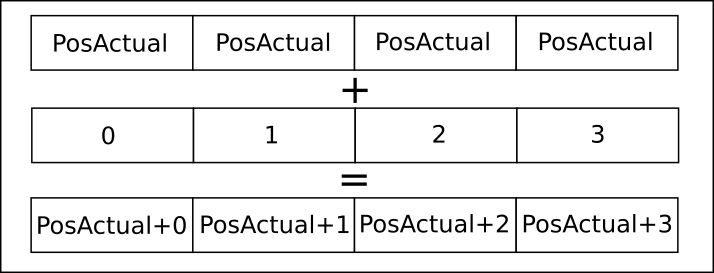
\includegraphics[scale=0.5]{imagenes/posActual.png} 
\end{center}

Luego, tanto para la posición (Pos) como para la altura (Size) de P1, se crean registros con la información replicada en cada int.

\begin{center}
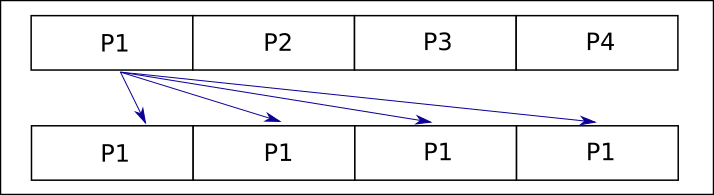
\includegraphics[scale=0.5]{imagenes/P1replicaInfo.png} 
\end{center}

Contamos con dos acumuladores, uno para la 'influencia' de los picos en esa posición y otro para la cantidad de picos que influyen. Para calcular el primero realizamos lo siguiente, donde Abs hace referencia a la función de valor absoluto:

\begin{center}
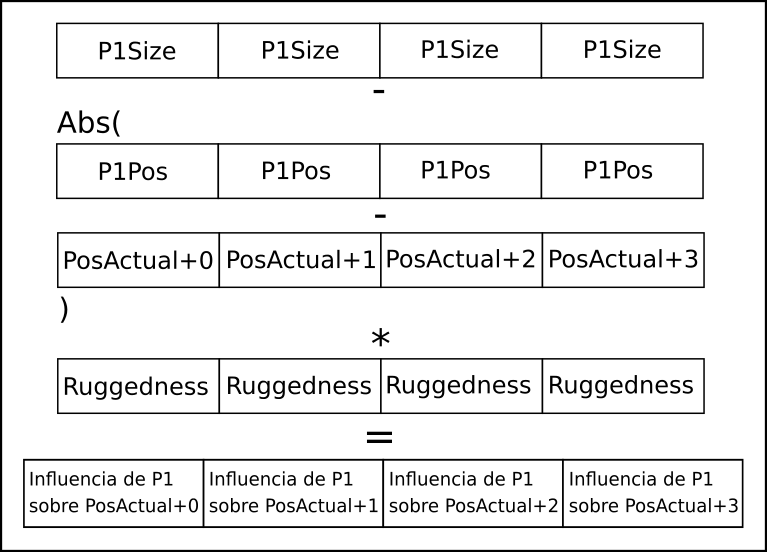
\includegraphics[scale=0.5]{imagenes/calculoInfluencia.png} 
\end{center}

Utilizando el registro que contiene la influencia obtenemos si el pico influye (influencia > 0) o no (caso contrario) sobre cada una de las cuatro posiciones.

Sumando esta información para cada pico obtenemos cuánta influencia, y de cuántos picos, tiene una posición determinada. Así al final del ciclo que recorre los picos solo nos queda dividir influencia por cantidad de picos y así obtenemos el valor real del terreno en la posición.
